\documentclass{article}

\usepackage{amsmath}
\usepackage{amssymb}
\usepackage{amsthm}
\usepackage[english]{babel}
\usepackage{graphicx}
\usepackage{natbib}
\usepackage{subfigure}
\usepackage{todonotes}
\usepackage[colorlinks=true,citecolor=blue,linkcolor=blue]{hyperref}
%\usepackage{icml2019}
\usepackage[accepted]{icml2019}

% autoref fix for Chapter
\addto\extrasenglish{%
  \renewcommand{\sectionautorefname}{Section}%
}

\newtheorem{proposition}{Proposition}
\newtheorem{lemma}[proposition]{Lemma}
\newtheorem{corollary}[proposition]{Corollary}
\newtheorem{theorem}[proposition]{Theorem}

\newcommand{\R}{\mathbb{R}}

\renewcommand{\P}{\mathcal{P}}
\newcommand{\U}{\mathcal{U}}
\newcommand{\X}{\mathcal{X}}
\newcommand{\indicator}[1]{\mathbf{1}\left[{#1}\right]}
\newcommand{\x}{\mathbf{x}}
\newcommand{\KL}[2]{D\left(#1 \middle\| #2 \right)}
\newcommand{\norm}[1]{\left\| #1 \right\|}
\newcommand{\ip}[2]{\left\langle #1, #2 \right\rangle}

\DeclareMathOperator*{\argmin}{argmin}
\DeclareMathOperator{\err}{err}
\DeclareMathOperator{\Exp}{\mathbf{E}}
\DeclareMathOperator{\VC}{VC}

\newcommand{\todoBalazs}[1]{\todo[backgroundcolor=blue]{Balazs: #1}}
\newcommand{\todoDavid}[1]{\todo[backgroundcolor=green]{David: #1}}
\newcommand{\todoSasha}[1]{\todo[backgroundcolor=orange]{Sasha: #1}}


% The \icmltitle you define below is probably too long as a header.
% Therefore, a short form for the running title is supplied here:
\icmltitlerunning{The information-theoretic value of unlabeled data in semi-supervised learning}

\begin{document}

\twocolumn[
\icmltitle{The information-theoretic value of unlabeled data in semi-supervised learning}

%\icmlsetsymbol{equal}{*}

\begin{icmlauthorlist}
\icmlauthor{Alexander Golovnev}{harvard}
\icmlauthor{D\'avid P\'al}{yahoo}
\icmlauthor{Bal\'azs Sz\"or\'enyi}{yahoo}
\end{icmlauthorlist}

\icmlaffiliation{harvard}{Harvard University, Cambridge, MA, USA}
\icmlaffiliation{yahoo}{Yahoo Research, New York, NY, USA}

\icmlcorrespondingauthor{D\'avid P\'al}{davidko.pal@gmail.com}

\icmlkeywords{semi-supervised learning, PAC learning, sample complexity, unlabeled data}

\vskip 0.3in
]

\printAffiliationsAndNotice{}

\begin{abstract}
We quantify the separation between the numbers of labeled examples required to
learn in two settings: Settings \emph{with} and \emph{without} the knowledge of
the distribution of the unlabeled data. More specifically, we prove a separation
by $\Theta(\log n)$ multiplicative factor for that the class of projections over
the Boolean hypercube of dimension $n$.

Learning with the knowledge of the distribution (a.k.a. \emph{fixed-distribution
learning}) can be viewed as an idealized scenario of semi-supervised learning
where the number of unlabeled data points is so great that the unlabeled
distribution is known exactly. For this reason, we call the separation the
\emph{value of unlabeled data}.
\end{abstract}

\begin{abstract}
We show a separation of the number of labeled examples required between learning
\emph{with} and \emph{without} the knowledge of the distribution of the
unlabeled data. For the class of projections over the Boolean hypercube of
dimension $n$, we show a separation by $\Theta(\log n)$ multiplicative factor.
For the class of monotone disjunctions over the Boolean hypercube of dimension
$n$, we show a separation by $\Theta(n)$ multiplicative factor. For the class of
halfspaces over $\R^n$, we show a separation by  $\Theta(n/\log n)$
multiplicative factor.

Learning with the knowledge of the distribution (a.k.a. \emph{fixed-distribution
learning}) can be viewed as an idealized scenario of semi-supervised learning
where the number of unlabeled data points is so great that the unlabeled
distribution is known exactly. For this reason, we call the separation the
\emph{value of unlabeled data}.
\end{abstract}


\section{Introduction}

\cite{Hanneke-2016} showed that for any class $C$ of Vapnik-Chervonenkis
dimension $d$ there exists an algorithm that $\epsilon$-learns any target
function from $C$ under any distribution from $O\left(\frac{d +
\log(1/\delta)}{\epsilon}\right)$ labeled examples with probability at least
$1-\delta$. For this paper, it is important to stress that Hanneke's algorithm
does \emph{not} receive the distribution of unlabeled data as input. On the
other hand, \cite{Benedek-Itai-1991} showed that for any class $C$ and any
distribution there exists an algorithm that $\epsilon$-learns any target from
$C$ from $O \left( \frac{\log N_{\epsilon/2} + \log (1/\delta)}{\epsilon}\right)$
labeled examples with probability at least $1-\delta$ where $N_{\epsilon/2}$ is the
size of an $\frac{\epsilon}{2}$-cover of $C$ with respect to the disagreement metric
$d(f,g) = \Pr[f(x) \neq g(x)]$. Here, it is important to note that Benedek-Itai
construct for each distribution a separate algorithm. In other words, they
construct a family of algorithms indexed by the (uncountably many) distributions
over the domain. Alternatively, we can think of Benedek-Itai's family of
algorithms as a single algorithm that receives the distribution as an input. It
is known that $N_\epsilon = O(1/\epsilon)^{O(d)}$; see \cite{Dudley-1978}. Thus,
ignoring $\log(1/\epsilon)$ factor, Benedek-Itai bound is never worse than
Hanneke's bound.

As we already mentioned, Benedek-Itai's algorithm receives as input the
distribution of unlabeled data. The algorithm uses it to construct an
$\frac{\epsilon}{2}$-cover. Unsurprisingly, there exist distributions which have
a small $\frac{\epsilon}{2}$-cover and thus sample complexity of Benedek-Itai's
algorithm on such distributions is significantly lower then the Hanneke's bound.
For instance, a distribution concentrated on a single point has an
$\frac{\epsilon}{2}$-cover of size $2$ for any positive $\epsilon$.

However, an algorithm does not need to receive the unlabeled distribution in
order to enjoy low sample complexity. For example, empirical risk minimization
(ERM) algorithm needs significantly less labeled examples to learn any target
under some unlabeled distributions. For instance, if a distribution is
concentrated on a single point, ERM needs only one labeled example to learn it.
One could be lead to believe that there exists an algorithm that does \emph{not}
receive the unlabeled distribution as input and achieves Benedek-Itai bound (or
a slightly worse bound) for \emph{every} distribution. In fact, one could think
that empirical risk minimization (ERM) or Hanneke's algorithm could be such
algorithm. If ERM, Hanneke's algorithm, or some other distribution-independent
algorithm had sample complexity that matches (or nearly matches) the optimal
distribution-specific sample complexity for \emph{every} distribution, we could
conclude that the knowledge of unlabeled data distribution is completely
useless.

As \cite{Darnstadt-Simon-Szorenyi-2013} showed this not the case. They showed
that \emph{any} algorithm for learning projections over $\{0,1\}^n$ that does
not receive the unlabeled distribution as input, requires, for some data
unlabeled distributions, more labeled examples than the Benedek-Itai bound.
However, they did not quantify this gap, beside stating that it grows without
bound as $n$ goes to infinity.

In this paper, we quantify the gap by showing that \emph{any}
distribution-independent algorithm for learning the class of projections over
$\{0,1\}^n$ requires, for some unlabeled distributions, $\Omega(\log n)$ times
as many labeled examples as Benedek-Itai bound. Furthermore, we show similar
results for the class of monotone disjunctions over the Boolean hypercube
$\{0,1\}^n$ where we show that any distribution-independent algorithm requires,
for some distributions, $\Omega(n)$ times as much labeled examples as the
Benedek-Itai bound. We show analogous result for halfspaces over $\R^n$, for
which we show that \emph{any} distribution-independent algorithm requires for
some unlabeled distributions $\Omega(\frac{n}{\log n})$ times as many labeled
examples as the Benedek-Itai bound.

\cite{Darnstadt-Simon-Szorenyi-2013} showed the gap for any class with
Vapnik-Chervonenkis dimension $d$ is at most $O(d)$. It is well known that
Vapnik-Chervonenkis dimensions of projections over $\{0,1\}^n$, monotone
disjunctions over $\{0,1\}^n$ and halfspaces over $\R^n$ are $\Theta(\log n)$,
$\Theta(n)$ and $\Theta(n)$ respectively. Thus our lower bounds match or almost
match the upper bound $O(d)$. However, it remains an open problem to close the
mismatch between $\Omega(\frac{n}{\log n})$ lower bound and $O(n)$ upper bound
for halfspaces over $\R^n$.

To better understand the relationship of the upper and lower bounds, we
illustrate the situation for the class of projections over $\{0,1\}^n$ in
Figure~\ref{figure:sample-complexity}. Recall that Vapnik-Chervonenkis dimension
of projections over $\{0,1\}^n$ is $\lfloor \log_2 n \rfloor$. This is a
folklore result, which we re-prove as
Proposition~\ref{proposition:vc-dimension-projections}.

\begin{figure}
\centering
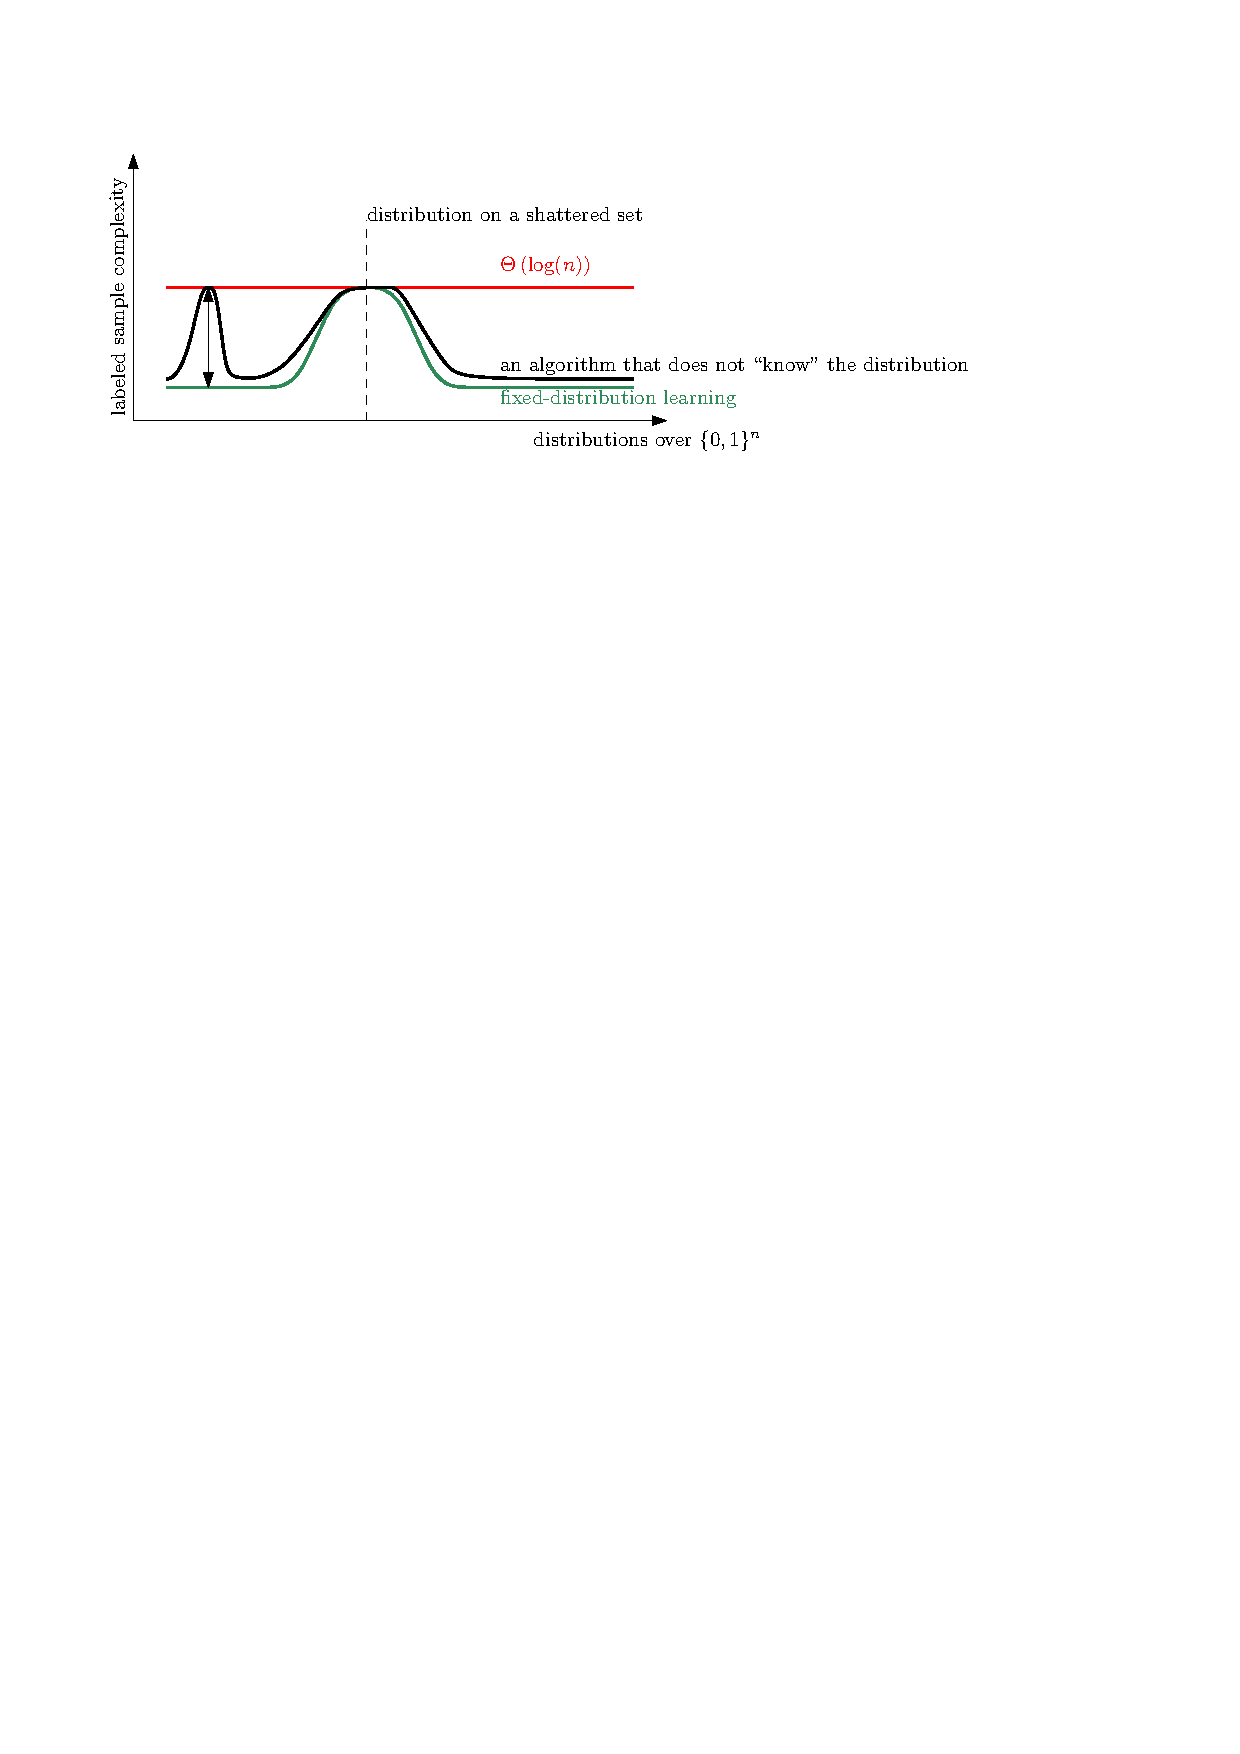
\includegraphics{figure}
\caption{\small The graph shows sample complexity bounds of learning a class of
projections over the domain $\{0,1\}^n$ under various unlabeled distributions.
We assume that $\epsilon$ and $\delta$ are constant, say, $\epsilon = \delta =
\frac{1}{10}$. The graph shows three lines. The red horizontal line is
Hanneke's bound for the class of projections, which is $\Theta(\VC(C_n)) =
\Theta(\log n)$. The green line is the Benedek-Itai bound. The green
line touches the red line for certain distributions, but is lower for other
distributions. In particular, for certain distributions the green line is
$O(1)$. The dashed line corresponds to a particular distribution on a shattered
set. This is where the green line and red line touch. Furthermore, here the
upper bound coincides with the lower bound for that particular distribution. The
black line is the sample complexity of an arbitrary
\emph{distribution-independent} algorithm. For example, the reader can think of
the ERM or Hanneke's algorithm.
We prove that there exist a distribution where the black line is
$\Omega(\log n)$ times higher than the green line. This separation is indicated
by the double arrow.}
\label{figure:sample-complexity}
\end{figure}

The paper is organized as follows. In \autoref{section:related-work} we review
prior work. \autoref{section:preliminaries} gives the necessary definitions and
basic probabilistic tools. Sections \ref{section:projections},
\ref{section:monotone-dijsunctions}, \ref{section:halfspaces} prove the
separation results for projections, monotone disjunctions, and halfspaces,
respectively. For completeness, in \autoref{section:epsilon-cover} we give a
proof of a simple upper bound $(e/\epsilon)^d$ on the size of the minimum
$\epsilon$-cover, and in \autoref{section:fixed-distribution-learning}, we re-prove
Benedek-Itai's $O \left( \frac{\log N_{\epsilon/2} + \log
(1/\delta)}{\epsilon}\right)$ sample complexity upper bound.

The proof technique in Sections \ref{section:projections}
\ref{section:monotone-dijsunctions}, \ref{section:halfspaces} is the same. The
differences only come up due to different combinatorial structure of the
three concept classes.

\section{Related Work}
\label{section:related-work}

The question of whether knowledge of unlabeled data distribution helps was
proposed and initially studied by \citet{Ben-David-Lu-Pal-2008}; see also
\citet{Lu-2009}. However, they considered only classes with Vapnik-Chervonenkis
dimension at most $1$, or classes with Vapnik-Chervonenkis dimension $d$ but
only distributions for which the size of the $\epsilon$-cover is
$\Theta(1/\epsilon)^{\Theta(d)}$, i.e. the $\epsilon$-cover is as large as it
can be.\footnote{For any concept class with Vapnik-Chervonenkis dimension $d$
and any distribution, the size of the smallest $\epsilon$-cover is at most
$O(1/\epsilon)^{O(d)}$. In fact, as we show in \autoref{section:epsilon-cover},
the size of the smallest $\epsilon$-cover is at most $(e/\epsilon)^d$.} In these
settings, for constant $\epsilon$ and $\delta$, the separation of labeled sample
complexities is at most a constant factor, which is exactly what
\citet{Ben-David-Lu-Pal-2008} proved. In these settings, unlabeled data are
indeed useless. However, these results say nothing about distributions with
$\epsilon$-cover of small size and it ignores the dependency on the
Vapnik-Chervonenkis dimension.

The question was studied in earnest by \citet{Darnstadt-Simon-Szorenyi-2013} who
showed two major results. First, they show that for any non-trivial concept
class $C$ and for every distribution, the ratio of the labeled sample
complexities between distribution-independent and distribution-dependent
algorithms is bounded by the Vapnik-Chervonenkis dimension. Second, they show
that for the class of projections over $\{0,1\}^n$, there are distributions
where the ratio grows to infinity as a function of $n$.

In learning theory, the disagreement metric and $\epsilon$-cover were introduced
by \citet{Benedek-Itai-1991} but the ideas are much older; see
e.g.~\citet{Dudley-1978, Dudley-1984}. The $O(1/\epsilon)^{O(d)}$ upper bound on
size of the smallest $\epsilon$-cover is by \citet[Lemma 7.13]{Dudley-1978}; see
also \citet[Chapter 4]{Devroye-Lugosi-2000} and \citet{Haussler-1995}.

For any distribution-independent algorithm and any class $C$ of
Vapnik-Chervonenkis dimension $d \ge 2$ and any $\epsilon \in (0,1)$ and $\delta
\in (0,1)$, there exists a distribution over the domain and a concept which
requires at least $\Omega \left(\frac{d + \log(1/\delta)}{\epsilon}\right)$
labeled examples to $\epsilon$-learn with probability at least $1 - \delta$;
see~\citet[Theorem 5.3]{Anthony-Bartlett-1999} and
\citet{Blumer-Ehrenfeucht-Haussler-Warmuth-1989,
Ehrenfeucht-Haussler-Kearns-Valiant-1989}. The proof of the lower bound
constructs a distribution that does \emph{not} depend on the algorithm. The
distribution is a particular distribution over a fixed set shattered by $C$. So
even an algorithm that knows the distribution requires $\Omega \left(\frac{d +
\log(1/\delta)}{\epsilon}\right)$ labeled examples.

\section{Preliminaries}
\label{section:preliminaries}

Let $\X$ be a non-empty set. We denote by $\{0,1\}^\X$ the class of all
functions from $\X$ to $\{0,1\}$. A \emph{concept class over a domain $\X$} is a
subset $C \subseteq \{0,1\}^\X$. A \emph{labeled example} is a pair $(x,y) \in
\X \times \{0,1\}$.

A \emph{distribution-independent learning algorithm} is a function
$A:\bigcup_{m=0}^\infty \left(\X \times \{0,1\} \right)^m \to \{0,1\}^\X$. In
other words, the algorithm gets as input a sequence of labeled examples $(x_1,
y_1), (x_2, y_2), \dots, (x_m, y_m)$ and outputs a function from $\X$ to
$\{0,1\}$. We allow the algorithm to output function that does not belong to
$C$, i.e., the algorithm can be improper. A \emph{distribution-dependent
algorithm} is a function that maps any probability distribution over $\X$ to a
distribution-independent algorithm.

Let $P$ be a probability distribution over a domain $\X$. For any two functions
$f:\X \to \{0,1\}$, $g:\X \to \{0,1\}$ we define the disagreement pseudo-metric
$$
d_P(f,g) = \Pr_{X \sim P}[f(X) \neq g(X)] \; .
$$
Let $C$ be concept class over $\X$, let $c \in C$, let $\epsilon, \delta \in (0,1)$.
Let  $X_1, X_2, \dots, X_m$ be an i.i.d. sample from $P$. We define the corresponding
labeled sample $T = ((X_1, c(X_1)), (X_2, c(X_2)), \dots, (X_m, c(X_m)))$.
We say that an algorithm $A$, \emph{$\epsilon$-learns} target $c$ from $m$ samples
with probability at least $1 - \delta$ if
$$
\Pr \left[d_P(c,A(T)) \le \epsilon \right]  \ge 1 - \delta \; .
$$

We recall the standard definitions from learning theory. For any concept $c:\X
\to \{0,1\}$ and any $S \subseteq \X$ we define $\pi(c,S) = \{x \in S ~:~ c(x) =
1 \}$. In other words, $\pi(c,S)$ is the set of examples in $S$ which $c$ labels
$1$. A set $S \subseteq \X$ is \emph{shattered} by a concept class $C$ if for
any subset $S' \subseteq S$ there exists a classifier $c \in C$ such that
$\pi(c,S) = S'$. \emph{Vapnik-Chervonenkis dimension} of a concept class $C$ is
the size of the largest set $S \subseteq \X$ shattered by $C$. A subset $C'$ of
a concept class $C$ is an \emph{$\epsilon$-cover} of $C$ for a probability
distribution $P$ if for any $c \in C$ there exists $c' \in C'$ such that
$d_P(c,c') \le \epsilon$.

To prove our lower bounds we need three general probabilistic results. The first
one is the standard Hoeffding bound. The other two are simple and intuitive
propositions. The first proposition says that if average error $d_P(c,A(T))$ is
high, the algorithm fails to $\epsilon$-learn with high probability. The second
proposition says that the best algorithm for predicting a bit based on some side
information, is to compute conditional expectation of the bit and thresholds it
at $1/2$.

\begin{theorem}[Hoeffding bound]
Let $X_1, X_2, \dots, X_n$ be i.i.d. random variables that lie in interval
$[a,b]$ with probability one and let $p=\frac{1}{n}\sum_{i=1}^n \Exp[X_i]$.
Then, for any $t \ge 0$,
$$
\Pr \left[{\frac {1}{n}} \sum_{i=1}^n X_i \ge p + t \right] \le e^{ - 2n t^2/(a-b)^2}  \qquad \text{and} \qquad
\Pr \left[{\frac {1}{n}} \sum_{i=1}^n X_i \le p - t \right] \le e^{ - 2n t^2/(a-b)^2}  \; . \\
$$
\end{theorem}

\begin{proposition}[Error probability vs. Expected error]
\label{proposition:error-probability-vs-expected-error}
Let $Z$ be a random variable such that $Z \le 1$ with probability one.
Then,
$$
\Pr[Z > t] \ge \frac{\Exp[Z] - t}{1 - t} \qquad \text{for any $t \in [0, 1)$.}
$$
\end{proposition}

\begin{proof}
We have
$$
\Exp[Z]
\le t \cdot \Pr[Z \le t] + 1 \cdot \Pr[Z > t]
= t \cdot (1 - \Pr[Z > t]) + \Pr[Z > t] \; .  \qquad \qedhere
$$
Solving for $\Pr[Z > t]$ finishes the proof.
\end{proof}

\begin{proposition}[Predicting Single Bit]
\label{proposition:single-bit}
Let $\U$ be a finite non-empty set. Let $U,V$ be random variables (possibly
correlated) such that $U \in \U$ and $V \in \{0,1\}$ with probability one. Let
$f:\U \to \{0,1\}$ be a predictor. Then,
$$
\Pr\left[ f(U) \neq V \right]
\ge \sum_{u \in \U} \left( \frac{1}{2} - \left| \frac{1}{2} -  \Exp \left[V \, \middle| \, U = u\right] \right| \right) \cdot \Pr[U = u] \; .
$$
\end{proposition}

\begin{proof}
We have
$$
\Pr \left[ f(U) \neq V \right] = \sum_{u \in \U} \Pr \left[ f(U) \neq V \, \middle| \, U = u \right] \cdot \Pr[U = u] \; .
$$
It remains to show that
$$
\Pr\left[ f(U) \neq V \, \middle| \, U = u \right]
\ge
\frac{1}{2} - \left| \frac{1}{2} -  \Exp \left[V \, \middle| \, U = u \right] \right| \; .
$$
Since if  $U=u$, the value $f(U) = f(u)$ is fixed, and hence
\begin{align*}
\Pr\left[ f(U) \neq V \, \middle| \, U = u \right]
& \ge \min\left\{ \Pr \left[ V = 1 \, \middle| \, U = u \right], \ \Pr \left[ V = 0 \, \middle| \, U = u \right] \right\} \\
& = \min\left\{ \Exp \left[ V  \, \middle| \, U = u \right], \ 1 - \Exp \left[ V \, \middle| \, U = u \right] \right\} \\
& = \frac{1}{2} - \left| \frac{1}{2} -  \Exp \left[ V  \, \middle| \, U = u \right] \right|
\end{align*}
We used the fact that $\min\{x, 1 - x\} = \frac{1}{2} - \left| \frac{1}{2} - x \right|$ for all $x \in \R$
which can be easily verified by considering two cases: $x \ge \frac{1}{2}$ and $x < \frac{1}{2}$.
\end{proof}


\bibliography{biblio}
\bibliographystyle{icml2019}

\appendix

\end{document}
